\documentclass[10pt,a4paper]{article}
\usepackage[utf8]{inputenc}
\usepackage{amsmath}
\usepackage{amssymb}
\usepackage{graphicx}
\usepackage{bm}
\usepackage{framed}
\author{Boon Han}
\title{Probability with Applications}
\begin{document}
    \maketitle
    \tableofcontents
    \newpage
    \section*{Edit Log (Changes from Original PDF)} % (fold)
    \label{sec:edit_log}
    \begin{enumerate}
      \item Sec 2.4(3) from $+ P(EF)$ to $- P(EF)$
      \item Sec 3 from $P(F) < 0$ to $P(F) > 0$
      \item Sec 3.2 from "iare" to "are"
      \item Sec 5.3 $F(a)$, added negative to exponent power
      \item Sec 8 Markov's Inequality, from $\leq$ to $\geq$
      \item Sec 5.4, Hazard Rate Function, changed t to t' and the bounds of the integral
    \end{enumerate}
    % section edit_log (end)
    \newpage
    \section{Combinatorial Analysis}
        \subsection{The Generalized Principle of Counting}
        A way to calculate the number of outcomes of $n_{i}$ experiments.
           \begin{framed}
               \center \textbf {The Generalized Principle of Counting} \\
               We do \emph{r} experiments. If the first will have n{\textsubscript{1}} possible outcomes and, for each of these n{\textsubscript{1}} outcomes there are n{\textsubscript{2}} outcomes of the second experiment, and for each possible outcome of the first two experiments there are n{\textsubscript{3}} possible outcomes... then there are a total of n{\textsubscript{1}} . n{\textsubscript{2}} ... n{\textsubscript{r}} total possible outcomes of the \emph{r} experiments.
           \end{framed}
           \subsection{Permutations}
           The number of ways to arrange $n$ objects where order matters.
               \begin{framed}
We can apply the generalized Principle of Counting to calculate the number of ways we can arrange \emph{n} objects. If, of $n$ objects, where $n_1$ are alike and $n_2$ are alike etc... then the number of ways to arrange them is $$ \frac{n!}{n_1!n_2!...n_r!} $$
               \end{framed}
            \begin{framed}
                \center \textbf{Permutations of n objects taken r at a time} \\
                If we have \emph{n} objects taken \emph{r} at a time, then \\
                1st object has \emph{n} outcomes; \\
                2nd object has \emph{n-1} outcomes; \\
                3rd object has \emph{n-2} outcomes; \\               
                ... \\
                r\textsuperscript{th} object has \emph{n-r+1} outcomes. \\
                So the number of permutations of n objects taken r at a time is$$ P_{n,r} = \frac{n!}{(n-r)!} $$
            \end{framed}
            \newpage 
            \subsection{Combinations}
            Permutations where order doesn't matter.
            \begin{framed}
                We can extend the concept of permuting n objects taken r at a time when the ordering within r does not matter. We remove repeated outcomes from P\textsubscript{n,r} to get the \textbf{Combination C\textsubscript{n,r}}: $$C_{n,r} = \binom{n}{r} =  \frac{n!}{r!(n-r)!} $$
            \end{framed}       
           A useful combinatorial identity is $$ \binom{n}{r} = \binom{n-1}{r-1} + \binom{n-1}{r} \qquad 1 \leq r \leq n $$
           Which states that, if we take an arbitrary object \emph{o}, then there are $\binom{n-1}{r-1}$ groups of size r that contain object \emph{o} and $\binom{n-1}{r}$ groups of size r that do not contain object \emph{o}.
           
           \subsection{The Binomial Theorem}
           \begin{framed}
               \center\textbf{The Binomial Theorem}
               $$(x+y)^n = \sum_{k=0}^{n}\binom{n}{k}x^ky^{n-k}$$
           \end{framed}
           
           \subsection{Multinomial Coefficients}
           \begin{framed}
               \center\textbf{Multinomial Coefficients} \\
               If $n_1 + n_2 + .. + n_r = n$ then we define: $$\binom{n}{n_1,n_2,...,n_r} = \frac{n!}{n_1!n_2!..n_r!}$$ which represents the number of possible divisions of n \textbf{distinct} objects into distinct groups of sizes $n_1$, $n_2$,...,$n_r$.
           \end{framed}
          \begin{framed}
          \center\textbf{The Multinomial Theorem}
          $$(x_1 + x_2 + ... + x_r)^n = \sum_{(n_1,...n_r):n_1+n_2+...+n_r = n}\binom{n}{n_1,n_2,...,n_r}x_1^{n_1}x_2^{n_2}...x_r^{n_r}$$
          The subtext of the summation means all values of $n_{i}$ have to sum up to $n$.
          \end{framed}
          \newpage
          \subsection{Number of Integer Solutions of Equations \\ (Bars and Stars Method)}
          Here we find a way to find the number of ways to satisfy the equation \\ $x_1 + x_2 + ... + x_r = n$. This is the same problem as trying to divide n indistinguishable objects into r nonempty groups. Since we choose $r-1$ of the $n-1$ possible spaces between objects there are $$\binom{n-1}{r-1} $$ possible selections which are \textbf{distinctly positive}. (IE $x_i > 0$) 
          If we want \textbf{distinct non-negative} values, then we find the solution to $y_1, y_2, ... y_r = n + r$ where $y_i = x_i + 1, i = 1,..,r$ and this gives us: $$ \binom{n+r-1}{r-1}$$
          If not all of n needs to be "used", then we can add a new variable on the LHS which will denote the amount of n "left out". 
          \subsection{Additional Information}
          \begin{table}[h]
                \centering
                \begin{tabular}{|l|l|}
                \hline
                \begin{tabular}[c]{@{}l@{}}Order Matters\\ Repetition Allowed                        \end{tabular}            & $n^r$ \\ \hline
                \begin{tabular}[c]{@{}l@{}}Order Matters\\ Repetition Not Allowed\end{tabular}        & $\frac{n!}{(n-r)!}$                   \\ \hline
                \begin{tabular}[c]{@{}l@{}}Order Doesn't Matter\\ Repetition Allowed\end{tabular}     & $\frac{n!}{r!(n-r)!}$                    \\ \hline
                \begin{tabular}[c]{@{}l@{}}Order Doesn't Matter\\ Repetition Not Allowed\end{tabular} & $\frac{(n+r-1)!}{(n-1)!}$                    \\ \hline
                \end{tabular}
            \end{table}
        \newpage
    \section{Axioms of Probability}
    Here we talk about the concept of probability of an event and show how probabilities can be computed.
    \subsection{Sample Space}
    We call the set of all possible outcomes of an experiment as the \emph{sample space} of an experiment. For example, for the experiment of the gender of a unborn child, the outcome sample space $S$ is $$ S = \{g,b\} $$ Any subset of this sample space is known as an \emph{event}. So if \emph{E} is the event that a girl is born, we can describe it as $$ E = \{g\} $$ More complex events can be described using the $\cup$ union or $\cap$ intersection symbols, where $E\cup F$ describes the event where either $E$ and $F$ occurs, while $E\cap F$ describes the event where both $E$ and $F$ occurs. For more than two events we have the equivalent $\bigcup_{n=1}^{\infty} E_n $ and $\bigcap_{n=1}^{\infty} E_n $ respectively. 
    \subsection{De Morgan's Laws}
    \begin{framed}
    \centering\textbf{De Morgan's Laws}
    $$ \Bigg( \bigcup_{i=1}^{\infty} E_i\Bigg)^c = \bigcap_{i=1}^{\infty} E_i^c  $$ $$\Bigg( \bigcap_{i=1}^{\infty} E_i\Bigg)^c = \bigcup_{i=1}^{\infty} E_i^c$$
    \end{framed}
    \subsection{Probability of an Event}
    \begin{framed}
        $$P(E) = \lim_{n \to \infty} \frac{n(E)}{n} $$ 
    \end{framed}
    \newpage
    \subsection{Simple Propositions}
    Here some propositions are listed. 
    \begin{framed}
        \begin{alignat}{3}
            &P(E^c) = 1 - P(E)  \\
            &\text{If } E \subset F  \text{ then }  P(E) \leq P(F)   \\
            &P(E \cup F) = P(E) + P(F) - P(EF) \\
            &P(E_1 \cup E_2 ... \cup E_n) = \sum_{i=1}^n P(E_i) - \sum_{i_1 < i_2} P(E_{i_1}E_{i_2}) + ... \\
            \nonumber  &+(-1)^{r+1} \sum_{i_1 < i_2 ... < i_r} P(E_{i_1} E_{i_2}...E_{i_r}) \\
            \nonumber &+...+ (-1)^{n+1}P(E_1 E_2 ... E_n)
        \end{alignat}  
    \end{framed}            
    An example of (4) is $P(E \cup F \cup G) = P(E) + P(F) +P(G) - P(EF) - P(EG) - P(FG) + P(EFG)$. Note that if we \textbf{assume equal probabilities} then we can simplify to something like $3.P(E) - 3.P(EF) + P(EFG)$. Note that due to the flipping nature of the addition / subtraction signs, the first term gives an upper bound on $P(E)$, the second gives a lower bound, the third gives upper, etc etc.
    \subsection{Equally Likely Outcomes}
    If we assume that all outcomes in a sample space $S$ are equally likely then we can conclude that $$P(E) = \frac{n(E)}{n(S)}$$
    \newpage
    \section{Conditional Probability and Independence}
    \begin{framed}
        \centering\textbf{Conditional Probability} \\
        If $P(F) > 0$, then $$P(E|F) = \frac{P(EF)}{P(F)}$$
    \end{framed}
    \begin{framed}
        \centering\textbf{The Multiplication Rule}
        $$P(E_1 E_2 ... E_n) = P(E_1)P(E_2 | E_1)P(E_3|E_1E_2)...P(E_n|E_1...E_{n-1})$$
    \end{framed}
    \subsection{Baye's Formula}
    Sometimes we cannot calculate the Probability of an event E directly. We instead calculate the conditional probability of E occuring based on whether or not a second event F has occured. Baye's Formula then allows us to derive $P(E)$ because:
    \begin{framed}
        \centering\textbf{Baye's Formula}
        $$P(E) = P(E|F)P(F) + P(E|F^c)(1-P(F))$$
    \end{framed}
\noindent If we we want to use this information to support a particular hypothesis, IE say that \textbf{This information E makes it more likely that an event has occured} then necessarily some conditions must hold. We know that 
    \begin{align*}
        P(H|E) &   = \frac{P(E|H)P(H)}{P(H)P(E|H) + P(H^c)P(E|H^c)} \\
        P(E|H)\uparrow \iff P(E|H) &\geq P(H)P(E|H) + P(H^c)P(E|H^c) \\
        \bm{P(E|H)} &\bm{\geq P(E|H^c)}
    \end{align*}
    In other words, an event $H$ is more likely after factoring some information $E$ if $E$ is more likely given $H$ than $H^c$. So if it is more likely [$P(E|H) \geq P(E|H^c)$] to have cancer ($H$) if you are a smoker ($E$) than not ($E^c$), then knowing that someone smokes increases the the probability that this person will have cancer. [$P(H|E) \uparrow$] \\
    In fact the change in probability of a hypothesis when a new evidence is introduced can be express compactly as the \emph{odds} of a hypothesis.
    \begin{framed}
        \centering\textbf{Odds of an Event A}
        $$\alpha = \frac{P(A)}{P(A^c)} = \frac{P(A)}{1-P(A)} $$
        Tells us how more likely it is that an event A occurs than it does not. If the odds are equal to $\alpha$, then we say that odds are ``$\alpha$ to 1" in favour of the hypothesis. \\
        The new odds after evidence $E$ is known, given a hypothesis $H$, is then a function of the old odds: 
        $$\frac{P(H|E)}{P(H^c|E)} = \frac{P(H)}{P(H^c)}\frac{P(E|H)}{P(E|H^c)}$$
    \end{framed}
    \newpage
    \subsection{Indepedent Events}
    We know from before that $P(E|F) = \frac{P(EF)}{P(F)}$. Generally we cannot simplify further. However, in the case that $E$ and $F$ do not depend on each other, we know that $P(E|F) = P(E)$. This can only happen if $E$ and $F$ are \textbf{independent}.
    \begin{framed}
        \centering\textbf{Independence} \\
        If two events are independent, then $P(EF) = P(E)P(F)$ \\
        It is also true that if $E$ and $F$ are independent, then so are $E$ and $F^c$
    \end{framed}
    If we have $n$ terms , these $n$ terms are independent only if every subset of these terms are independent. For example,
    \begin{framed}
        \centering\textbf{Independence of Three Events} \\
        \centering Three events $E$, $F$, $G$ are independent only if 
        \begin{align*}
            P(EFG) &= P(E)P(F)P(G)   \\
            P(EF) &= P(E)P(F)  \\
            P(FG) &= P(F)P(G) \\
            P(EG) &= P(E)P(G) 
        \end{align*}
        Note that there are $2^n$ subsets, so if we exclude subsets of size 1 (trivially, $P(E) = P(E)$) and size 0 (null set), we have $2^n - n - 1$ subsets to consider.
    \end{framed}
    \newpage
    \section{Random Variables}
    A random variable $X$ is a variable whose possible values describe the possible numeric outcomes of a random phenomenon. So, for a dice roll, $P(X = 1) = \frac{1}{6}$.
        \begin{framed}
            \centering\textbf{Cumulative Distribution Function}
            $$F(x) = P(X \leq x) \qquad -\infty < x < \infty$$
        \end{framed}
        \subsection{Discrete Random Variables}
            \begin{framed}
                \centering\textbf{Probability Mass Function $p$}
                $$p(a) = P\{X = a\}$$ 
                $p(a)$ is a \emph{positive number} (not function) for a countable number of values of a, and is $0$ otherwise.
                Note that because we are dealing with probabilities,
                $$\sum_{i=1}^{\infty}p(x_    i) = 1$$
                \centering\textbf{Cumulative Distribution Function $F$}
                $$F(a) = \sum_{\text{all } x \leq a} p(x)$$
                Note that $F(a)$ is a step function where the value is constant at intervals and then takes a jump at certain points. \\
                \centering\textbf{Expected Value}
                $$E[X] = \sum_{x:p(x) > 0} xp(x)$$
                A weighted average of the possible values X can take, weighted by its probability.
            \end{framed}
            \newpage
        \subsection{Expectation of Function of Discrete Random Variable}
        \begin{framed}
            \centering\textbf{Expectation of a Function of a Random Variable}
                $$E[g(X)] = \sum_ig(x_i)p(x_i)$$
                Note that $x_i$ is replaced with $g(x_i)$. \\
                Consequently, we also can say that: 
                $$E[aX + b] = aE[X] + b $$
                $$E[X^n] = \sum_{x:p(x)>0}x^np(x)$$
        \end{framed}
        
        \subsection{Variance}
        A measure of the deviation of a random variable from its mean.
       \begin{framed}
       	\centering\textbf{Variance}
       	    $$Var(X) = E[(X-\mu)^{2}]$$ 
       	    $$Var(X) = E(X^{2}) - E(X)^{2}$$
       	    $$Var(aX + b) = a^{2}Var(X)$$
       \end{framed}
       \subsection{Bernoulli and Binomial Random Variables}
       \begin{framed}
       	\centering\textbf{Bernoulli Random Variable ($n$, $p$)    } \\
       	An single experiment whose outcome can be classified as either a \emph{success} or \emph{failure}. \\ The probability mass function $p(a)$ is given by $$p(0) = P\{X=0\} = 1- p$$ $$p(1) = P\{X=1\} = p$$
       \end{framed}
       \begin{framed}
               	\centering\textbf{Binomial Random Variable ($n > 0$ , $0 < p < 1$)} \\
               	$n$ independent bernoulli random variables with probability of success $p$ are carried out. X represents \textbf{number of successes} in $n$ trials. \\
               	The probability mass function $p(i)$ is given by:
               	$$p(i) = \binom{n}{i}p^{i}(1-p)^{n-i} \qquad i=0,1,...,n $$
               \end{framed}
               \newpage 
               \begin{framed}
               	\centering\textbf{Properties of Binomial Random Variables}
               	$$E[X] = np$$
               	$$Var(X) = np(1-p)$$
               	If X is a binomial Random Variable with parameters $n$ and $p$, where $0 < p < 1$ then as $k$ goes from 0 to $n$, $P\{X=k\}$ first increases monotonically and then decreases monotonically, reaching its largest value when $k$ is the largest integer $\leq (n+1)p$.
               \end{framed}
               \begin{framed}
               	\centering\textbf{Calculating the Binomial Distribution Function} \\
               	To calculate the cumulative distribution function of a Binomial RV(\emph{n}, \emph{p}) $P\{X \leq i\}$, we use the known relationship:
               	$$P\{X=k+1\} = \frac{p}{1-p}\frac{n-k}{k+1}P\{X=k\}$$
               	We can start with $P\{X=0\}$ and then derive the $k+1$ term recursively.
               \end{framed}
               \subsection{Poisson Random Variable}
               A good estimation to the Binomial Random Variable if $n$ is large and $p$ is small such that $np$ is of moderate size. In this case, $\lambda = np$. 
               \begin{framed}
               	\centering\textbf{Poisson Random Variable($\lambda > 0$)}
                  $$p(i) = P\{X=i\} = e^{-\lambda}\frac{\lambda^{i}}{i!} \qquad i=0,1,2...$$ $\lambda$ is also the Expected number of successes.
               	
               \end{framed}
               The following are some Random Variables that fit a Poisson RV. The common theme is that all of them have a large $n$ but a small $p$.
               \begin{enumerate}
               \item The number of misprints on a book
               \item Number of people in a community that live to 100
               \item Number of wrong telephone numbers that are dialed a day
               \item Number of packages of dog biscuits sold in a particular store every day
               \item etc...
               \end{enumerate}
               \newpage 
               \begin{framed}
               	\centering\textbf{Computing the Poisson Random Variable}
               	$$\frac{P\{X=i+1\}}{P\{X=i\}}=\frac{e^{-\lambda}\lambda^{i+1}/(i+1)!}{e^{-\lambda}\lambda^{i}/i!}=\frac{\lambda}{i+1}$$
               	and we can start with $P\{X=0\} = e^{-\lambda}$ and compute successive $P\{X=a\}$ since $$P\{X=i+1\} = \frac{\lambda}{i+1}P\{X=i\}$$
               \end{framed}
               \begin{framed}
               	\centering\textbf{Properties of Poisson Random Variables}
               	$$E(X) = \lambda$$
               	$$Var(X) = \lambda$$
               \end{framed}
               	\subsection{Geometric Random Variable}
               	A binomial random variable with consecutive failures and terminates on its first success. X is the number of trials required to get this success.
               	\begin{framed}
               		\centering\textbf{Geometric Random Variable ($ 0 < p < 1$)}
               		$$P\{X=n\} = (1-p)^{n-1}p \qquad n=1,2,...$$
               		Note that in the Binomial RV, $n$ is fixed while $i$ is the variable denoting number of successes. Here, $n$ is the variable.
               	\end{framed}
               	\begin{framed}
               		\centering\textbf{Properties of Geometric Random Variables}
               		$$E(X) = \frac{1}{p}$$
               		$$Var(X) = \frac{1-p}{p^{2}}$$
               	\end{framed}
               	\newpage 
               	\subsection{Negative Binomial Random Variable}
               	A Binomial Random Variable that terminates when $r$ successes are accumulated. In essence, we have a Binomial Random Variable modelling the first $r-1$ successes, followed by a terminating success with probability $p$.
               	\begin{framed}
               		\centering\textbf{Negative Binomial Random Variable ($r \in \mathbb{R}^{+}$, $p$)}
               		$$P\{X=n\} = \binom{n-1}{r-1}p^{r}(1-p)^{n-r} \qquad n=r,r+1...$$
               		Note that the \textbf{geometric random variable} is just a negative binomial with $r=1$.
               	\end{framed}
               	\begin{framed}
               		\centering\textbf{Propeties of a Negative Binomial}
               		$$E(X) = \frac{r}{p}$$
               		$$Var(X) = \frac{r(1-p)}{p^{2}}$$
               	\end{framed}
               	\subsection{Hypergeometric Random Variable}
               	A binomial RV requires independence between experiments. If $p$ changes based on the ratio of two binary elements, such as when we have a urn of $N$ balls, $m$ white and $N-m$ black, the "successes" is described as follows:
               	\begin{framed}
               		\centering\textbf{Hypergeometric Random Variable ($n, N, m$)}
               		$$P\{X=i\} = \frac{\binom{m}{i}\binom{N-m}{n-i}}{\binom{N}{n}} \qquad i=0,1,...,n$$
               		Very simply, we use the generalized counting principle to count $i$ "successes", $n-i$ failures conditioned on the fact that we drew $n$ samples.
               	\end{framed}
               	\begin{framed}
               		\centering\textbf{Properties of Hypergeometric Random Variables}
               		$$E[X] = \frac{nm}{N}$$
               		$$Var(x) = np(1-p)(1-\frac{n-1}{N-1})$$
               		$$Var(x) \approx np(1-p) \qquad \text{when N is large w.r.t n}$$
               		Intuitively, a Hypergeometric RV approximates a Binomial RV for large N w.r.t n because if the sample drawn is small, the probabilities \emph{remain almost constant}
               	\end{framed}
               	\newpage 
               	\subsection{Expected Value of Sums of Discrete Random Variables}
               	\begin{framed}
               		\centering\textbf{Linearity of Expectations}
               		$$E\bigg[\sum^{n}_{i=1}X_{i}\bigg] = \sum^{n}_{i=1}E[X_{i}]$$
               	\end{framed}
               	\subsection{Properties of the Discrete Cumulative Distribution Function}
               	The Cumulative Distribution Function denotes the probability that a random variable takes on a value \emph{less than or equal to b}.
               	\begin{enumerate}
               	\item F is non-decreasing function
               	\item $\lim_{b \to \infty}F(b) = 1$
               	\item $\lim_{b \to -\infty}F(b) = 0$
               	\item F is right continuous. 
               	\item $P\{a < X \leq b\} = F(b) - F(a) \qquad \forall a,b.a < b$
               	\end{enumerate}
               	\newpage 
    \section{Continuous Random Variables}
    As opposed to \emph{discrete} random variables whose set of possible values is either finite or countably infinite,  there exist random variables whose set of possible values is \textbf{uncountable}. This gives rise to \emph{continuous random variables}. We are concerned with the probability that the RV is within a set of values $B$.
    \begin{framed}
    	\centering\textbf{Probability Density Function f}
    	$$f(x) = P\{X=a\}$$
    	where $f$ is some continuous function.
    \end{framed}
    
    \begin{framed}
    	\centering\textbf{Cumulative Distribution Function F}
    	 $$P\{X\in B\} = \int_{B}f(x) dx$$      
    	 $$P\{a \leq X \leq b\} = \int_a^bf(x)dx$$
        $$P\{X < a\} = P\{X \leq a\} = F(a) = \int_{-\infty}^{a}f(x)dx$$
        Note that $P\{X < a\} = P\{X \leq a\}$ because $\int_{a}^{a}f(x) = 0$.
    \end{framed}
    \begin{framed}
    	\centering\textbf{Relationship between F and f}
    	$$\frac{d}{da}F(a) = f(a) $$
    	The derivative of the Cumulative Distribution Function is the Probability Density.
    \end{framed}
    \begin{framed}
    	\centering\textbf{Properties of Continuous Random Variables}
    	$$E[X] = \int_{-\infty}^{\infty}xf(x)dx$$
    	$$E[g(X)] = \int_{-\infty}^{\infty}g(x)f(x) dx$$
    	$$E[aX+b] = aE[X] + b$$
    	$$Var(X) = E[X^{2}]-(E[X])^{2}$$
    	$$Var(aX + b) = a^{2}Var(X)$$
    \end{framed}
    \newpage 
   \subsection{Uniform Random Variables}
   A continuous random variable is uniform if its probability within an interval is constant, and zero otherwise.
    \begin{framed}
    	\centering\textbf{Uniform Random Variable $(\alpha, \beta)$} \\
    	A random variable is uniformly distributed over an interval $(\alpha, \beta)$ if
    	$$f(x)  = \begin{cases}
    	        \frac{1}{\beta - \alpha} \qquad \alpha < x < \beta\\
    	        0 \qquad \text{otherwise}
    	    \end{cases}$$
    	$$F(a)  = \begin{cases}
    	        0 \qquad a \leq \alpha \\
    	        \frac{a - \alpha}{\beta - \alpha} \qquad \alpha < x < \beta\\
    	        1 \qquad \alpha \geq \beta
    	    \end{cases}$$    
    \end{framed}    
    \begin{framed}
             	      		\centering\textbf{Properties of Uniform Random Variables}
             	      		$$E[X] = \frac{\beta + \alpha}{2}$$\\
             	      		$$Var(X) = \frac{(\beta - \alpha)^{2}}{12}$$
    \end{framed}
    \subsection{Normal Random Variables}
    A random variable whose probability density follows a bell-curve shape.
    \begin{framed}
    	\centering\textbf{Normal Random Variable $(\mu, \sigma^{2})$}
    	$$f(x) = \frac{1}{\sqrt{2\pi}\sigma}e^{-(x-\mu)^{2}/2\sigma^{2}} \qquad -\infty < x < \infty$$ 
    	\centering\textbf{Standardized Normal Random Variable} \\
    	A normally distributed random variable X can be standardized: $Z = \frac{X - \mu}{\sigma}$ which is normally distributed with parameters $\mu = 0, \sigma^{2} = 1$ such that $$\Phi(x) = \frac{1}{\sqrt{2\pi}}\int^{x}_{-\infty}e^{-y^{2}/2}dy$$
    	such that we can represent the Cumulative Distribution Function $F_{X}(a)$ as:
    	      		$$F_{X}(a) =P\{X \leq a\} = \Phi\bigg(\frac{a-\mu}{\sigma}\bigg)$$
    \end{framed}       
    \newpage 
    \begin{framed}
    	      		\centering\textbf{Properties of a Normal Random Variable} 
    	      		$$E[X] = \mu$$
    	      		$$Var(X) = \sigma^{2}$$
    	      		$$E[aX + b] = a\mu + b$$
    	      		$$Var(aX + b) = \alpha^{2}\sigma^{2}$$
    \end{framed}
    The following theorem is to estimate a binomial random variable using a normal approximation. This works when n is large. 
    \begin{framed}
    	\centering\textbf{The DeMoivre-Laplace Limit Theorem} \\
    	If $S_{n}$ denotes the number of successes in a binomial experiment then the "standardized" $S_{n}$ is approximated by a standard normal random variable: $$P\bigg\{a \leq \frac{S_{n}-np}{\sqrt{np(1-p)}} \leq b\bigg\} \to \Phi(b) - \Phi(a)$$ as n $\to$ $\infty$.\\
    	 Since we are applying a continuous RV to estimate a discrete RV, we apply \emph{continuity correction}. $$If P\{X=20\} \to_{c.corr} P\{19.5 \leq X < 20.5\}$$ Then we \textbf{normalize} the $S_{n}$ terms ($19.5 \text{ and } 20.5$) and use the standardized normal RV $\Phi$. $$\Phi(b) - \Phi(a) = \Phi(\frac{19.5 - 20}{\sqrt{10}}) - \Phi(\frac{20.5 - 20}{\sqrt{10}})$$
     \end{framed}
     \subsection{Exponential Random Variables}
     An Exponential Random Variable is used to model the amount of time until a specific event occurs.
     \begin{framed}
     	\centering\textbf{Exponential Random Variable ($\lambda$)}
     	The Exponential RV Probability Density is given as:
     	$$f(x) = \begin{cases}
     	\lambda e^{-\lambda x} \qquad \text{if } x \geq 0 \\
     	0 \qquad \qquad \text{if } x < 0
     	\end{cases}$$
     	$$F(a) = 1 - e^{-\lambda a} \qquad a \geq 0 $$
     \end{framed}
     \newpage 
     \begin{framed}
     	\centering\textbf{Properties of Exponential Random Variables}
     	$$E[X] = \frac{1}{\lambda}$$
     	$$Var(X) = \frac{1}{\lambda^{2}}$$
     	$$\text{Memoryless: } P\{X > s + t | X > t\} = P\{X > s\} \quad \text{for all }s,t \geq 0$$ 
     	$$\text{Equivalently: } P\{X > s + t\} = P\{X > s\}P\{X > t\}$$
     \end{framed}
     \subsection{Hazard Rate Functions}
     The Hazard Rate Function is the conditional probability that a $t$-unit-year-old item will fail at time $t'$ given that it already survived up to $t$. \\
     For example, the death rate of a person who smokes is, at each age, twice that of a non-smoker.
     \begin{framed}
     \centering\textbf{Survival Function}
     $$\text{Survival Function } = 1-F(t)$$
     	\centering\textbf{Hazard Rate Functions} \\
     	A ratio of the probability density function to survival function.
     	$$\lambda (t) = \frac{f(t)}{\bar{F}(t)}$$
     	The parameter $\lambda$ of an exponential distribution is often referred to as the \textbf{rate }of the distribution.\\
     	The failure rate function for the exponential distribution uniquely determines the distribution $F$.\\
     	In general, $$F(t) = 1 - exp \bigg\{-\int_{0}^{t}\lambda(t) dt\bigg\}$$
     	For example, if a random variable has a hazard rate function $$\lambda (t) = a + bt$$ then the cumulative distribution function $F(t)$ is $1 - e^{-(at+bt^{2}/2)}$ and differentiation will yield the density $$f(t) = (a+bt)e^{-(at+bt^{2}/2)} \qquad t \geq 0$$
     \end{framed}
     \section{Jointly Distributed Random Variables}
     We now extend probability distributions to two random variables.
     \begin{framed}
     	\centering\textbf{Jointly Distributed Random Variables}
     	$$F(a,b) = P\{X \leq a, Y \leq b\} \qquad -\infty < a,b < \infty$$
     	We can obtain marginal distribution of X from the joint distribution F easily:
     	$$F_{X}(a) = F(a,\infty)$$
     	And we can answer all joint probability statements about X and Y because: $$P\{a_{i} < X \leq a_{2}, b_{1} < Y \leq b_{2}\} = F(a_{2},b_{2}) + F(a_{1},b_{1}) - F(a_{1},b_{2}) - F(a_{2}, b_{1})$$
     \end{framed}
     \begin{framed}
     	\centering\textbf{Discrete Jointly Distributed Random Variables}
     	The discrete case is modelled with the \emph{joint probability mass function} by $$p(x,y) = P\{X=x,Y=y\}$$ and marginals (example of X, with trivial equivalent for Y) $$p_{X}(x) = \sum_{y:p(x,y)>0}p(x,y)$$ Note that we can represent the joint probability mass function best in table form.
     \end{framed}
     \begin{framed}
     	\centering\textbf{Continuous Jointly Distributed Random Variables} The     continuous case is modelled by (note there are two variables) $$P\{(X,Y) \in C\} = \iint_{(x,y) \in C} f(x,y)\ dxdy$$
     	$$P\{X \in A, Y \in B\} = \int_{B}\int_{A}f(x,y)\ dxdy$$ $$F(a,b) = \int_{-\infty}^{b}\int_{-\infty}^{a}f(x,y)\ dxdy$$ $$f(a,b) = \frac{\partial^{2}}{\partial a \  \partial b}F(a,b)$$ $$f_{X}(x) = \int_{-\infty}^{\infty}f(x,y)\ dy \qquad \text{with trivial equivalent for y}$$
     \end{framed}
     \newpage 
     \subsection{Independent Random Variables}
     Here we discuss the situation where knowing the value of one Random Variable does not affect the other.
     \begin{framed}
     	\centering\textbf{Independence of Jointly Distributed Random Variables}
     	Two Random Variables are \emph{independent} if $$P\{X \in A, Y \in B\} = P\{X \in A\}P\{Y \in B\}$$ Consequently, we can say $$P\{X \leq a, Y \leq b\} = P\{X \leq a\}P\{Y \leq b\}$$ Hence, in terms of joint distribution, X and Y are independent if $$F(a,b) = F_{X}(a)F_{Y}(b) \qquad \text{for all } a,b$$ For the discrete case we have $$p(x,y) = p_{X}(x)p_{Y}(y) \qquad \text{for all } x,y$$ and for the continuous case we have $$f(x,y) = f_{X}(x)f_{Y}(y) \qquad \text{for all } x,y$$ The continuous (discrete) random variables X and Y are independent if and only if their joint probability density(mass) functions can be expressed as follows: $$f_{X,Y}(x,y) = h(x)g(y) \qquad -\infty < x < \infty, -\infty < y < \infty$$
     Note that independent is symmetric. Consequently, if its difficult to determine independece in our direction, it is valid to go the other way.
     \end{framed}
     \begin{framed}
     	\centering\textbf{Conditional Distribution: Discrete Case} \\
     	Conditional Probabillity Mass Function of $X$ given $Y=y$
     	$$p_{X|Y}(x|y) = \frac{p(x,y)}{p_{Y}(y)}$$
     	Conditional Probability Distribution Function of $X$ given $Y=y$
     	$$F_{X|Y}(x|y) = \sum_{a\leq x}p_{X|Y}(a|y)$$
     	If $X$ and $Y$ are independent then then $$p_{X|Y}(x|y) = P\{X=x\}$$
     \end{framed}
     \newpage 
     \subsection{Conditional Distribution: Continuous Case}
     \begin{framed}
     \centering\textbf{Conditional Density Function}
     $$f_{X|Y}(x|y) = \frac{f(x,y)}{f_{Y}(y)}$$
     \centering\textbf{Conditional Probabilities of Events}
     $$P\{X \in A | Y = y\} = \int_{A}f_{X|Y}(x|y)\ dx$$
     \centering\textbf{Conditional Cumulative Distribution Function of X (with trivial equivalent for Y)}
     $$F_{X|Y}(a|y) = \int_{-\infty}^{a}f_{X|Y}(x|y)\ dx$$
     A conditional probability such as $P\{X > 1 | Y = y\}$ is a function with variables x and y.
    \end{framed}
    \subsection{Multinomial Distribution}
    A multinomial distribution arises when $n$ independent and identical experiments are performed. We have $n$ random variables, and we denote number of experiments with outcome $i$ with the random variable $X_{i}$.
    \begin{framed}
    	\centering\textbf{The Multinomial Distribution}
    	$$P\{X_{1}=n_{1}, X_{2}=n_{2}...X_{r}=n_{r}\} = \frac{n!}{n_{1}!n_{2}!...n_{r}!}p_{1}^{n_{1}}p_{2}^{n_{2}}...p_{r}^{n_{r}} $$
    \end{framed}
    \section{Properties of Expectation}
    \subsection{Expectation of Sum of Random Variables}
    \begin{framed}
    	\centering\textbf{Discrete Case}
    	    $$E[g(X,Y)] = \sum_{y}\sum_{x}g(x,y)p(x,y)$$
    	\centering\textbf{Continuous Case}
    	    $$E[g(X,Y)] = \int_{-\infty}^{\infty}\int_{-\infty}^{\infty}g(x,y)f(x,y)\ dxdy$$
    \end{framed}
    \newpage 
    \subsection{Covariance, Variance of Sums, and Correlations}
    \begin{framed}
    	\centering\textbf{Expectation of Product of Independent Variables} \\
    	If X and Y are independent, then
    	    $$E[g(X)h(Y)] = E[h(Y)]E[g(X)]$$
    \end{framed}
    \begin{framed}
    	\centering\textbf{Covariance between X and Y} \\
    	The Covariance between X and Y gives us information about the relationships about the two RV. 
    	\begin{align*}
    	Cov(X,Y) &= E[(X - E[X])(Y - E[Y])] \\
    	              &= E[XY] - E[X]E[Y]
    	\end{align*}
    	Note that if $X$ and $Y$ are independent, then $Cov(X,Y) = 0$. However, the converse is not true.\\
    	There are some things to note:
    	\begin{enumerate}
    	 \item $Cov(X,Y) = Cov(Y,X)$
    	 \item $Cov(X,X) = Var(X)$
    	 \item $Cov(aX,Y) = aCov(X,Y)$
    	 \item $Cov\bigg(\sum^{n}_{i=1}X_{i}, \sum^{m}_{j=1}Y_{j}\bigg) = \sum_{i=1}^{n}\sum_{j=1}^{m}Cov(X_{i}, Y_{j})$
    	 \end{enumerate} 
    \end{framed}
    \begin{framed}
    	\centering\textbf{Variance of multiple Random Variables} \\
    	In general,
    	 $$Var\bigg(\sum_{i=1}^{n}X_{i}\bigg) = \sum_{i=1}^{n}Var(X_{i}) + 2 \sum\sum_{i<j}Cov(X_{i},X_{j})$$
    	 If $X_{1},...,X_{n}$ are pairwise independent, meaning each event is independent of \emph{every other possible combination} of paired events, then $$Var\bigg(\sum_{i=1}^{n}X_{i}\bigg) = \sum_{i=1}^{n}Var(X_{i})$$
    	 Note that mutual independence is pairwise independence with the additional requirement that $P(A \cap B \cap ...) = P(A) \times P(B) \times ...$
    \end{framed}
    \newpage 
    \begin{framed}
    	\centering\textbf{Correlation} \\
    	A measure of linearity between two Random Variables. A value near +1 or -1 indicates high degree of linearity, while a value near 0 indicates otherwise.\\
    	As long as $Var(X)Var(Y)$ is positive, the correlation between X and Y is defined as $$\rho(X,Y) = \frac{Cov(X,Y)}{\sqrt{Var(X) Var(Y)}}$$ and $-1 \leq  \rho(X,Y) \leq 1$
    \end{framed}
    \subsection{Conditional Expectation}
    We extend Expectations to the case where we involve conditional probabilities.
    \begin{framed}
    	\centering\textbf{Discrete Case}
    	$$E[X|Y=y] = \sum_{x}xp_{X|Y}(x|y)$$ 
    	\centering\textbf{Continuous Case}
    	$$E[X|Y=y] = \int_{-\infty}^{\infty}xf_{X|Y}(x|y)\ dx$$
    	\centering\textbf{Computing Expectations by Conditioning} \\
    	If we denote $E[X|Y]$ to be the function of the random variable Y whose value at $Y=y$ is $E[X|Y=y$, then $$E[X] = E[E[X|Y]]$$
    	In the discrete case, $$E[X] = \sum_{y}E[X|Y=y]P\{Y=y\}]$$
    	$$E[X] = \int_{-\infty}^{\infty}E[X|Y=y]f_{Y}(y)\ dy$$
    	This allows us to easily compute expectations by first conditioning on some appropriate variable.
    \end{framed}  	 	   
    \newpage 
    \subsection{Computing Probabilities by Conditioning}
    We extend the computation of probabilities to conditional statements.
    \begin{framed}
    \centering\textbf{Discrete Case}
    $$P(E) = \sum_{y}P(E|Y=y)P(Y=y)$$ 
    \centering\textbf{Continuous Case}
    $$P(E) = \int_{-\infty}^{\infty}P(E|Y=y)f_{Y}(y)\ dy$$
\end{framed}
\subsection{Moment Generating Functions}
Moments of a random variable X (Expectations of the powers of X) can be calculated using Moment Generating Functions:
$$M(t) = E[e^{tX}]$$
\begin{framed}
	\centering\textbf{Discrete Case, X has mass function $p(x)$}
	$$M(t) = \sum_{x}e^{tx}p(x)$$
	\centering\textbf{Continuous Case, X has density function $f(x)$}
	$$M(t) = \int_{-\infty}^{\infty}e^{tx}f(x)\ dx$$
	We do this by differentiating $n$ times and evaluating at $t=0$ to get the expectation of the $n^{th}$ moment. For Example, $$M'(0) = E[X]$$
\end{framed}
\newpage 
\begin{figure}[h]
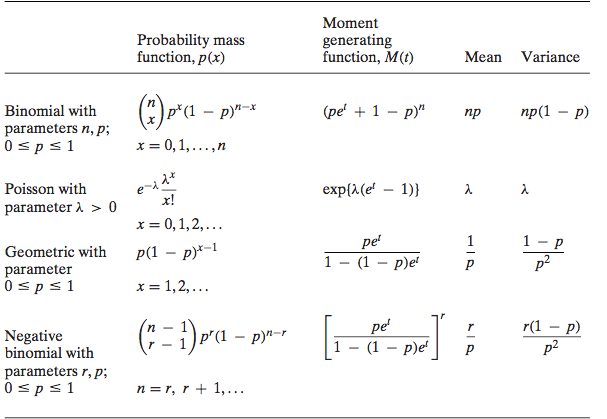
\includegraphics[width=\columnwidth]{Images/discrete_momgenf.png}   
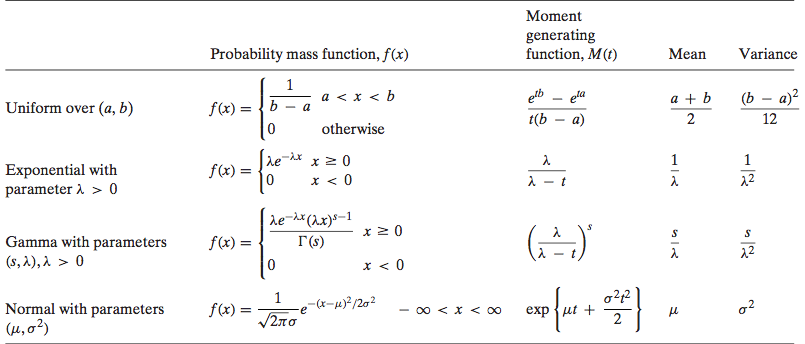
\includegraphics[width=\columnwidth]{Images/continuous_momgenf.png}      	
\end{figure}   	
\newpage    	 	      	    
\section{Limit Theorems}
Here we study some important conclusions of probability theory. Markov's and Chebyshev's inequalities allow us to derive bounds on probabilities when only the mean, or both mean and variance, of the probability distribution are known. 
\subsection{Markov's Inequality}
If X is a random variable that takes only non-negative values then for any $a > 0$,
$$P\{X \geq a\} \leq \frac{E[X]}{a}$$
\subsection{Chebyshev's Inequality}
If X is a random variable with finite mean $\mu$ and variance $\sigma^{2}$ then for any $k \geq 0$, $$P\{|X-\mu|\geq k\} \leq \frac{\sigma^{2}}{k^{2}}$$
\subsection{Chernoff's Bounds}
If X is a random variable with $M_{x}(t) = E[e^{tX}]$ then 
$$P(X \geq a) \leq e^{-ta}M_{x}(t) \qquad \text{for all } t \geq 0$$   
$$P(X \leq a) \leq e^{-ta}M_{x}(t) \qquad \text{for all } t < 0$$ 
\subsection{Weak Law of Large Numbers}
The weak law of large numbers (also called Khintchine's law) states that the sample average converges in probability towards the expected value.\\
Let $X_{1}, X_{2}, ..., X_{n}$ be a sequence of independent and indentically distributed random variables, each with finite mean $E[X] = \mu$. Then for any $\epsilon > 0$, $$P\bigg\{\bigg|\frac{X_{1} + ... + X_{n}}{n}-\mu\bigg| \geq \epsilon \bigg\} \to 0 \qquad \text{as } n \to \infty$$
\subsection{Strong Law of Large Numbers}
Let $X_{1}, X_{2}, ..., X_{n}$ be a sequence of independent and indentically distributed random variables, each with finite mean $E[X] = \mu$. Then, with probability 1, $$\frac{X_{1} + X_{2} + ... + X_{n}}{n} \to \mu \qquad \text{as } n \to \infty$$ 
\newpage 
\subsection{Central Limit Theorem}
The Central Limit Theorem provides a simple method to compute approximate probabilities of sums of independent random variables.
\begin{framed}
	\centering\textbf{Central Limit Theorem} \\
	Let $X_{1}, X_{2}, ..., X_{n}$ be a sequence of independent and indentically distributed random variables, each with mean $\mu$ and variance $\sigma^{2}$. Then the distribution $$\frac{X_{1}, ..., X_{n} - n\mu}{\sigma\sqrt{n}}$$ tends to the standard normal as $n \to \infty$. So $$P\bigg\{\frac{X_{1}, ..., X_{n} - n\mu}{\sigma\sqrt{n}} \leq a\bigg\} \to \frac{1}{\sqrt{2\pi}}\int_{-\infty}^{a}e^{-x^{2}/2}\ dx \qquad \text{as } n\to\infty$$
\end{framed}
\newpage 
\section{Markov Chains}
Markov Chains model a system of N states where there is a probability of moving from one state to another at every click of a clock. The probability of moving to state  $i$ to state $j$ depend entirely on $i$ and not the number of clock "clicks" passed. $$P_{i,j} = P(\text{system is in state } j \text{ at time } n+1| \text{ system in state } i \text{ at time } n)$$ Such probabilities are written in a \emph{transition matrix}. $$P = \begin{bmatrix}
    P_{0,0} & P_{0,1} & P_{0,2} \\
    P_{1,0} & P_{1,1} & P_{1,2} \\
    P_{2,0} & P_{2,1} & P_{2,2}
\end{bmatrix}$$ where $P_{i,j}$ is the probability of transitioning from state $i$ to state $j$ at this time.\\
The $n^{th}$ probability vector $\pi^{(n)}$ is a vector of the probabilities that we are in state $i$ at time $n$, where $$\pi^{(n)} = \big(\pi^{(n)}_{0},\pi^{(n)}_{1},\pi^{(n)}_{2}\big)$$
\begin{framed}
	\centering\textbf{Properties of the $n^{th}$ probability vector}
	$$\pi^{(n+1)} = \pi^{(n)}P $$
	$$\pi^{(n)} = \pi^{(0)}P^{n}$$
\end{framed}
For large $n$, if $\lim_{n \to\infty}\pi^{(n)}$ exists and is independent of $\pi^{0}$ then $$\pi = \lim_{n \to \infty} \pi^{(n)}$$ is the \textbf{steady state probability vector}. It can be found by:
\begin{enumerate}
\item Solving for $\pi = \pi P$ 
\item Use $\pi_{0} + ... + \pi_{N-1} = 1$
\end{enumerate} assuming it exists (ergodic). It \textbf{may not} if
\begin{enumerate}
\item Periodic Behaviour where the chain goes back and forth
\item Traps where a chain gets stuck in one state or another, in which case it depends on $\pi^{(0)}$
\end{enumerate}
\begin{framed}
	\centering\textbf{Ergodic Markov Chain}
	A markov chain is ergodic iff there exists $n \in \mathbb{N}^{+}$ such that $P^{n}$ has no zero entries. It is aperiodic and irreducible. \\
	If so, then the \textbf{steady state probability vector} exists and $\pi$ is independent of $\pi^{(0)}$.
\end{framed}
\newpage 
    \section{Markov Chains in Continuous Time}
    If, instead of a system changing at discrete times, it can change at any time, and the time between transitions are \emph{exponentially distributed}, then the transitional rate probabilities are given by a \textbf{Poisson Process}.  Here we focus on calculate the resulting steady state probability vector.
    \subsection{Poisson Process}
    We can model things like the number of buses $\tilde{N}(t)$ arriving in a time period $[t, t+\sigma t]$. This Poisson Process has some properties:
    \begin{framed}
\centering\textbf{Properties of a Poisson Process $\tilde{N}(t)$}
\begin{enumerate}
\item For any fixed $t$, $\tilde{N}(t)$ is a discrete random variable
\item $\tilde{N}(0) = 0$, so counting starts at time 0
\item \# of events in disjoint intervals are independent
\item $\tilde{N}(t + h) - \tilde{N}(t)$ = \# of events in $[t,t+h]$ for $h \to 0$
\item $P(\tilde{N}(h)=1) = P(\text{event occurs in $[t,t+h]$)}$ = $\lambda h + E(h) \text{as } \frac{E(h)}{h}\to 0, h \to 0$ \qquad $E(h)$ is small even in relation to $h$
\item $\frac{1}{h}P(\tilde{N}(h) \geq 2) \to 0 \qquad \text{as } h \to 0$
\end{enumerate}
If the above are satisfied then $$P(\tilde{N}(t) = k) = \frac{(\lambda t)^{k}}{k}e^{-\lambda t} \qquad k=0,1,2,...$$
\end{framed}
\subsection{Birth Death Process}
A special case of continuous time Markov Chains where within some small time period $\delta t$ transitions can only increase the state variable by 1.
\begin{framed}
	\centering\textbf{Birth Rates}
	$\lambda_{i,i+1}=b_{i}$\\
	\centering\textbf{Death Rates}
	$\lambda_{i,i-1}=d_{i}$ \\
	otherwise $\lambda_{i,j} = 0$ \\
	If each $b_{i}$ and $d_{i}$ is non-zero, and N is finite, then the steady state probability vector exists and it is independent of $\pi^{(0)}$
	\end{framed}
	\newpage 
	\begin{framed}
		\centering\textbf{Calculating Steady State Probability Vector for a Birth-Death Process} \\ In general, 
		$$b_{j}\pi_{j} = d_{j+1}\pi_{j+1} \qquad j=0,1,2...,N-1$$ 
		\begin{enumerate}
		\item $\pi_{j} = \frac{b_{0}b_{1}...b_{j-1}}{d_{0}d_{1}...d_{j-1}}\pi_{0} \qquad j=1,2,...,N-1$
		\item $1 = \pi_{0} + \pi_{1} + ... + \pi_{N-1}$ 
		\end{enumerate}
\end{framed}
\begin{framed}
	\centering\textbf{M/M/S Queues}
	Birth-Death Processes with particular choice of birth rates and death rates and in infinite number of possible states (length of the queue).
	\begin{enumerate}
	\item Customers arrive as described by Poisson Process with rate $\lambda$.
	\item $S = \#$ of servers
	\item Service time of Server (time to service a customer) exponentially distributed with mean $\frac{1}{\mu}$
	\item State 'j' mean $j$ customers are in queue, $j = 0,1,2...$
	\item The actual state: discrete $J \in \{0,1,...,N-1\}$
	\item $b_{j}= \lambda \qquad j = 1,2,...,S$
	\item $d_{j} = \begin{cases}
	j\mu, \qquad j=1,2,...,S \\
	S\mu, \qquad j \geq S
	\end{cases}$
	\end{enumerate}
	If $\lambda < S_{\mu}$ then a steady state distribution $\pi = (\lambda_{0},\lambda_{1},...)$ exists, and is independent of $\pi^{(0)}$. \\ $\pi_{j}$ is the Probability Mass Function of state J: $P(\text{J customers in queue}\}$
\end{framed}
Following page describes the steady state probability vector of \textbf{M/M/1}, the mean queue length and an example.
\newpage 
\begin{figure}[ht] 
\includegraphics[width=\columnwidth]{Images/MM1.png} 
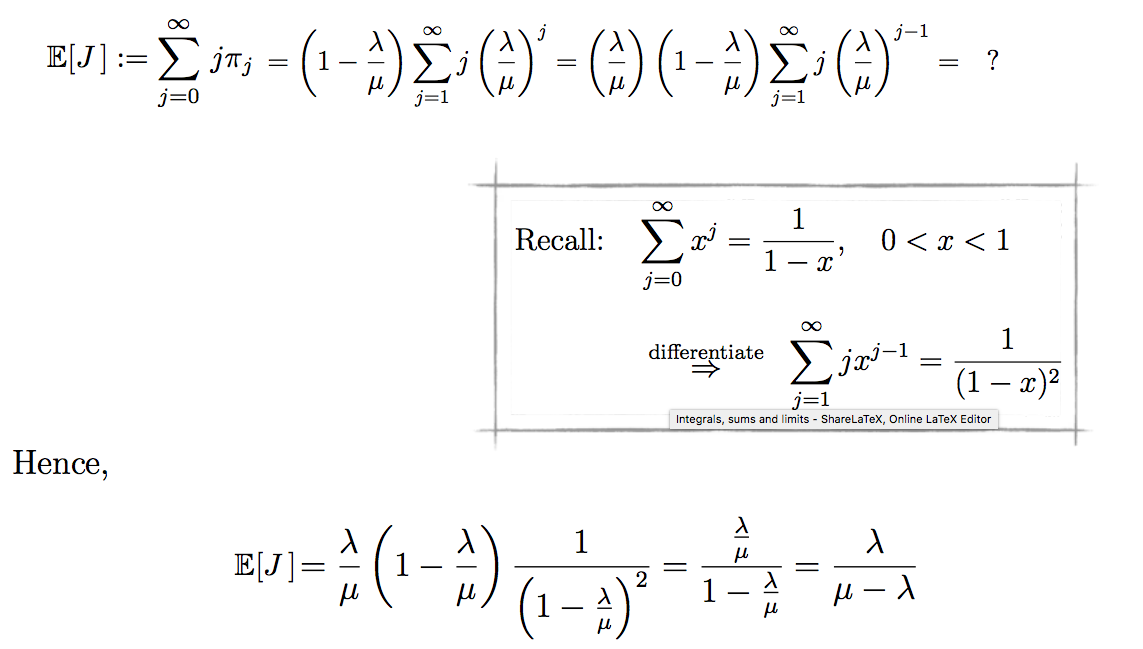
\includegraphics[width=\columnwidth]{Images/MeanQueueLength.png} 
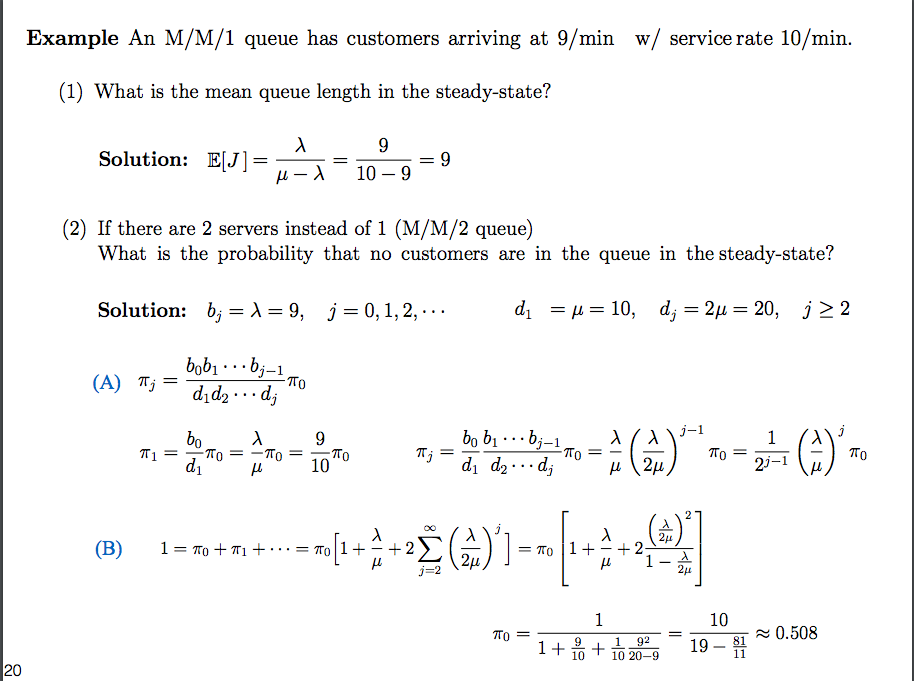
\includegraphics[width=\linewidth]{Images/MMS_EG.png} 
\end{figure}
\begin{figure}[ht]
                \centering
                \includegraphics[width=\linewidth]{"Images/zscore_table"}
\end{figure}  		      	
\end{document}
